%------------------------------------------------------------
%
\documentclass{llncs}%
\usepackage{quotes}
\usepackage{epstopdf}
\usepackage{bsymb}
\usepackage{alltt}
\usepackage{amsmath}%
\usepackage{graphicx}
\usepackage{hyperref}
\usepackage{enumitem}
\usepackage{amssymb,amsfonts,textcomp}
\usepackage{color}
%-------------------------------------------
\begin{document}
%
\title{An Experience Report on Event-B Code Generation, from an Industry-led Assessment of the Event-B Approach }
\author{A. Edmunds\inst{1}, C. Snook\inst{1}, K. Wiederaenders\inst{2} and K. Reichl\inst{2}}

\institute{University of Southampton, UK\\
\and Thales Transportation Systems, Germany
}


\maketitle
%
\begin{abstract}
This report describes the experience of our participation in an industry-led assessment of Rodin/Event-B, and Tasking Event-B for code generation. The feasibility study involved the modelling of controller software, and the operating environment, of a simple fan controller. The aim of the study was to evaluate the complete Event-B methodology, from abstract specification to Java implementation. During the project various tool enhancements were completed, and a list of feature requests was created by the industrial partner. The list may serve to influence the direction of research, or the commercialisation of the tool. In the report we also draw some general conclusions, including how the collaboration brought to light some interesting differences between the goals of academia and industry. 
 \end{abstract}
%
%
\section{Overview}
Rodin is a  tool platform for the rigorous specification of critical systems, using the Event-B approach~\cite{ABR10}. The tool was developed in the RODIN project~\cite{RodinTool}, and experience with industry was gained in the DEPLOY project~\cite{DEPLOY}. However, code generation (specifically our version, which we call Tasking Event-B~\cite{ae2011a}) was not assessed by industry in any depth. The collaboration reported in this paper is the first such undertaking, that we are aware of, that seeks to evaluate the seamless development from abstract specification to Java implementation, using Tasking Event-B in an industrial setting. The tool enhancements, reported here, have been partly funded by the ADVANCE project~\cite{advance}, and in part by the industrial partner.

In the remainder of this section we present the industrial collaborator's motivation for the study, and give an overview of Event-B, Tasking Event-B and code generation. Where necessary, we illustrate the text with example fragments from the case-study. In Sect.\ref{translat} we discuss translation of Tasking Event-B to code. In Sect.~\ref{CaseStudy} we present more details of the case study. In Sect.~\ref{Experience} we provide a commentary on our experience; and in Sect.~\ref{Learning} we summarize the lessons learned.
%
\subsection{Motivation for the Case-Study}
At the beginning of the collaboration, a brief (2 week) period of Event-B training was provided, with additional consolidation time. Then a case study was proposed, so that the industrial partner could assess the feasibility of using Event-B and Tasking Event-B in a larger project, by undertaking a small, but complete, development (from abstract specification to Java implementation). The industrial partner had an existing implementation, for comparison. They also wished to assess some of the other plug-ins, such as the ProB animator/model checker~\cite{ProB}, and a related plug-in for model-based testing~\cite{DBLP:conf/asm/DincaIMS12}. We will not report these results here. 

The criteria for the case study was that it should be small enough to be completed in 3 months (whilst still being near the start of the Event-B learning curve). It was to cover as many aspects of Event-B development as possible. This included the use of Rodin platform, with proof, and refinement. Use of decomposition and composition~\cite{decomp2010c}; iUML-B state-machines~\cite{snookIUMLB}; the theory plug-in for language specification~\cite{ecs18269}. We also needed to develop a Java interface to the environment; and use the Eclipse Java Development Tool-kit, so that the generated code could be run in the Eclipse environment~\cite{EclipseOrg} without further editing. 
%
%
\subsection{Event-B}
%
The Event-B method~\cite{ABR10} was developed by J.R. Abrial, and uses set-theory, predicate logic and mathematical constructs to model discrete systems. Event-B \emph{machines} are used to describe dynamic properties of a system, and \emph{contexts} the fixed properties. Properties (such as safety-properties) are described in a machine's \emph{invariants} and a context's \emph{axioms}.  Machines are able to use contexts by adding them to the \emph{sees} clause; then content of a Context is visible and accessible to a machine. Machines describe the dynamic aspects of a system using state variables, and guarded atomic \emph{events}. Events can have non-deterministic parameters, which can be interpreted as a kind of local variable, or (as we do in code generation for Tasking Event-B) actual and formal parameters for methods and their calls. Proof obligations are generated by the tool automatically. They represent the conditions that should be satisfied, to demonstrate that the model is consistent with the specified properties. Discharging proof obligations (proving their truth) shows that the related properties hold. In many cases proof obligations are discharged by Rodin's automatic proof tools, but it is often necessary to perform interactive proof within Rodin. Interactive proof is undertaken by suggesting strategies, and sub-goals in the form of hypotheses. 

A fragment of an Event-B specification is shown in Fig.~\ref{fig:TextualEventB}, with more shown in Appendix~\ref{abst}. Variables are introduced in the variables clause, and typed in the \textbf{invariant}. Invariants also describe desired safety properties. An initialisation event occurs before all others, Fig.~\ref{fig:TextualEventB2}. The initial state can be specified using deterministic or non-deterministic assignments, $\bcmeq$ or $\bcmin$ resp.  The \emph{read} event refines some abstract \emph{read} event, and declares a parameter \emph{p1}, which is used in the \textbf{where} clause. Other event guards may also appear here. After initialisation, any enabled event with all its guards true may occur. State updates are specified in the \textbf{then} (action) clause using deterministic or non-deterministic assignments, or the event may do nothing (\emph{skip}). Event-B also incorporates diagrammatic means of specification. One such approach is that of state-machine diagrams~\cite{snookIUMLB}. Fig.~\ref{fig:sm1} shows a state-machine diagram, which is a preview of the one used in our case-study.  
%
%
%
\begin{figure}
\centering
\begin{minipage}{0.9\linewidth}
\textcolor{blue}{MACHINE} FanCtrlMachine 

\textcolor{blue}{SEES} FanCtrlMachine\_implicitContext, FanCtrlContext 

\textcolor{blue}{VARIABLES} C\_tempPSU, C\_tempAmbient, \ldots \ \  \ 

\textcolor{blue}{INVARIANTS}

\ \ C\_tempPSU ${\in}$ $\mathbb{Z}$  ${\wedge}$ C\_tempAmbient ${\in}$ $\mathbb{Z}$  ${\wedge}$ C\_fanSpeed ${\in}$ $\mathbb{Z}$ \ldots ${\wedge}$ \ 

\ \ (Controller = Normal $\Rightarrow $ \

 \ \ ((C\_tempPSU ${\geq}$ HWM\_PSU) ${\vee}$ (C\_tempAmbient ${\geq}$
HWM\_AMBIENT)\

\ \ \quad $\Rightarrow $ C\_fanOn = TRUE)) ${\wedge}$\ \  \ 

\ \ (Controller = Normal $\Rightarrow $ \dots
\end{minipage}
	\caption{Example of Event-B with Invariants}
	\label{fig:TextualEventB}
\end{figure}
%
%
%
\begin{figure}[t]
\centering
\begin{minipage}{0.45\linewidth}
INITIALISATION:\ \ 

THEN

\ \ C\_tempPSU :${\in}$ $\mathbb{Z}$ 

\ \ C\_tempAmbient :${\in}$ $\mathbb{Z}$ 

\ \ \ldots

END

\bigskip

\end{minipage}
%
\begin{minipage}{0.45\linewidth}
write: 

REFINES write 

ANY p1\ \  \ 

WHERE

\ \ p1 = C\_fanOn \ \ 

THEN

\ \ E\_MAX6650\_fanOn $:=$ p1 

END
\end{minipage}
\caption{Example Event-B Events}
\label{fig:TextualEventB2}
\end{figure}
%
%
%
\begin{figure}[b]
\centering
\includegraphics[width=0.9\textwidth]{sm1.png}
\caption{Fan Controller Event-B State-machine Diagram}\label{fig:sm1}
\end{figure}
%

Refinement is the process of adding detail to a development. A refinement machine can introduce new variables, invariants, and events. New and existing events can modify new variables, but there are restrictions on how existing variables are modified. Consistency in the relationship between an abstract machine and its refinements is maintained by discharging the automatically generated proof obligations. An example of a refined machine can be seen in Appendix~\ref{refi}.    

Shared Event-B decomposition~\cite{Butler09a,decomp2010b} is a technique that we use to handle complexity; we are able to split a single machine specification into several. We begin with partitioning variables into machines. After decomposition the events that refer to them are shared between machines. The shared events are said to synchronize: i.e. only enabled when both events are enabled. Fig.~\ref{fig:Decomp2} shows a diagram, where event $e$ is decomposed, into $e_a$ and $e_b$. The events can be recomposed; in~\cite{ae2011a} we describe the synchronization of two events as being equivalent to a single, merged, atomic event. Each event consists of guards and actions, and $e$ can be represented as a guarded command: $g \rightarrow a$. The composition, using this notation, is $g \rightarrow a \triangleq g_a \land g_b \rightarrow a_a~ ||~ a_b$. In this case $g_a$ is the guard of $e_a$ and so on; in this situation we use the parallel action operator $||$ where the operands are actions. Event Synchronization uses shared parameters to facilitate communication between machines.  A composed machine construct is generated~\cite{decomp2010c}, that keeps track of the artefacts after decomposition. As we move towards towards implementation, the decomposed artefacts reflect entities in the implementation; which assists with code generation.
%
\begin{figure}[t]
\centering
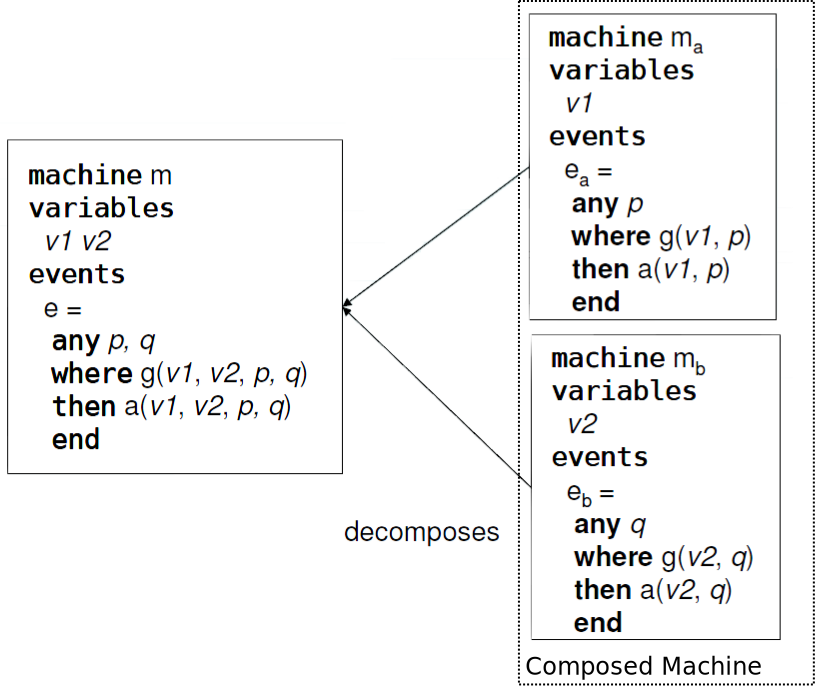
\includegraphics[width=0.6\textwidth]{Decomp2.png}
\caption{Shared Event Decomposition}
\label{fig:Decomp2}
\end{figure}
%
\subsection{Tasking Event-B}\label{TEB}
Tasking Event-B incorporates an implementation level specification language, which, when added to a machine, describes how to translate an Event-B machine into an implementation. Annotations are added to machines and contexts. These provide additional, implementation-level details, to guide the code generator. In this way machines can be implemented as task/thread-like constructs; shared, monitor-like constructs; or provide simulations of the environment. These annotations can be translated back into to Event-B, to provide a model of the implementation, and are also translated to their related constructs in an implementation. The machine \emph{Type} annotations are \emph{AutoTask}, \emph{Shared} and \emph{Environ} respectively.  In embedded systems, AutoTask Machines typically model \emph{controller} tasks (of the implementation). 

The AutoTask, shown in Fig.~\ref{fig:TaskBody}, allows us to specify a task type; which can be either periodic, single-shot, triggered, or repeating. In the figure we see a value, in milliseconds, for the period. In a \emph{task-body} we can specify an ordering of events. We can use sequential, branching and looping operators. In the example, we state that the \emph{write} event takes place, followed by the \emph{read} event. Both synchronize with their counterpart events in the environment. The \emph{output} clauses provides feedback via the console during a simulation. In an implementation, if there is a state-machine associated with an AutoTask machine, it is evaluated before the task-body.
%
\begin{figure}
\centering
\begin{minipage}{0.5\textwidth}
\textcolor{blue}{TASKING} MACHINE TYPE AutoTask \ 

\ \ TASK TYPE Periodic PERIOD 100 \ 

\ \ TASK BODY

\ \ \ \ write ;

\ \ \ \ read ;

\ \ \ \ output C\_fanSpeed: C\_fanSpeed ;

\ \ \ \ output C\_fanOn: C\_fanOn 

\textcolor{blue}{END}
\end{minipage}
\caption{A Task Body}
\label{fig:TaskBody}
\end{figure}
%
%
%
%
%
\section{ Translation to Code}\label{translat}
Event-B and Tasking Event-B provide the information used to generate code. There are code generators for translations to Java, Ada and OpenMP C, which make use of the theory plug-in~\cite{ecs18269}. The theory plug-in allows us to specify a mapping between Event-B mathematical operators, and their implementation counterparts, for each target language. We then use a pattern matching feature, where the translation is performed. AutoTask, shared, and environ machine translations, introduced in the last section, are hard-coded. In this report we focus on Java translations, at the request of our industrial collaborators. 

There is a formal definition of the relationship between Event-B with Tasking Event-B, and implementation constructs; details are given in~\cite{ae2011a}. But, an intuitive explanation is to describe the implementation as a refinement of the formal model. For the task body clause, in Tasking Event-B, sequences map to sequences of program statements. The branching statement $IF~e_a ~ELSE~e_b$, with events $e_a$ and $e_b$ map to a conditional statement where the event guards become branch conditions, and event assignment actions become assignment statements. The code fragment of Fig.~\ref{fig:FanContV} shows the implementation of the fan-controller task, the details are shown in context in Appendix~\ref{ContJava}.
%
%
%
\begin{figure}
{\ttfamily
\ \ \textbf{\textcolor{blue}{public}} \textbf{\textcolor{blue}{void}}
run()\{}

{\ttfamily
\ \ \ \ \textbf{\textcolor{blue}{while}}(true)}

{\ttfamily
\ \ \ \ \{} \ldots

{\ttfamily
\ \ \ \ \ \ ((ControllerNewImpl)MainEntry.}

{\ttfamily
\ \ \ \ \ \ \ \ getTask(``ControllerNewImpl '')).ControllerstateMachine();}

{\ttfamily
\ \ \ \ \ \ ((EnvNewImpl)MainEntry.getTask(``EnvNewImpl '')).write(C\_fanOn);}

{\ttfamily
\ \ \ \ \ \ if ((Controller != Normal))}

{\ttfamily
\ \ \ \ \ \ \{}

{\ttfamily
\ \ \ \ \ \ \ \ Pointer{\textless}Integer{\textgreater}
C\_fanSpeedPointer = new Pointer{\textless}Integer{\textgreater}();}

{\ttfamily
\ \ \ \ \ \ \ \ Pointer{\textless}Integer{\textgreater}
C\_tempAmbientPointer = new Pointer{\textless}Integer{\textgreater}();}

{\ttfamily
\ \ \ \ \ \ \ \ Pointer{\textless}Integer{\textgreater}
C\_tempPSUPointer = new Pointer{\textless}Integer{\textgreater}();}

{\ttfamily
\ \ \ \ \ \ \ \ ((EnvNewImpl)MainEntry.getTask( ``EnvNewImpl ''))}

{\ttfamily
\ \ \ \ \ \ \ \ \ \ .read(C\_fanSpeedPointer, C\_tempAmbientPointer,\

\ \ \ \ \ \ \ \ \ \ \ C\_tempPSUPointer);}

{\ttfamily
\ \ \ \ \ \ \ \ C\_fanSpeed = C\_fanSpeedPointer.value;}

{\ttfamily
\ \ \ \ \ \ \ \ C\_tempAmbient = C\_tempAmbientPointer.value;}

{\ttfamily
\ \ \ \ \ \ \ \ C\_tempPSU = C\_tempPSUPointer.value;}

{\ttfamily
\ \ \ \ \ \ \}}

{\ttfamily
\ \ \ \ \ \ System.out.println(``C\_fanSpeed: '' + C\_fanSpeed);}

{\ttfamily
\ \ \ \ \ \ System.out.println(``C\_fanOn: '' + C\_fanOn);}

{\ttfamily
\ \ \ \ \ \ {\dots} }
\caption{Code Generated from the Fan Controller Task-body}
\label{fig:FanContV}
\end{figure}
The task body is implemented in the \emph{run} method of a Java thread. The method has code for forcing the thread to sleep, if the period has not been reached. The scheduling of threads in this way was considered sufficient for the purposes of this feasibility study. The state-machine code is in the \emph{ControllerstateMachine} method. After this is invoked, the result (the command to turn the fan on/off) is written to the environment using the \emph{write} method call. This is followed by a \emph{read} method call, where the latest environment values are read.  The environment implementation (not presented here) simulates a temperature rise when the fan is off, and is lowered when the fan is on. A fragment of the state-machine implementation is shown in Fig.~\ref{fig:StateM} to give a flavour of the generated code.
%
\begin{figure}[t]
{\ttfamily
\textbf{\textcolor{blue}{public}} \textbf{\textcolor{blue}{void}}
ControllerstateMachine()\{}

{\ttfamily
\ \textbf{\textcolor{blue}{switch}}(Controller)\{}

{\ttfamily
\ \textbf{\textcolor{blue}{case}} Step:}

{\ttfamily
\ Controller = Control;}

{\ttfamily
\ \textbf{\textcolor{blue}{break}};}

{\ttfamily
\ \textbf{\textcolor{blue}{case}} Control:}

{\ttfamily
\ \textcolor{blue}{if} ((!((C\_tempPSU {\textgreater}=
HWM\_PSU) {\textbar}{\textbar} (C\_tempAmbient {\textgreater}= HWM\_AMBIENT))) }

{\ttfamily
\ \ \ \&\& (!((C\_tempPSU {\textless}= LWM\_PSU) \&\&
(C\_tempAmbient {\textless}= LWM\_AMBIENT))))}

{\ttfamily
\ \{}

{\ttfamily
\ \ Controller = Normal;}

{\ttfamily
\ \}}

{\ttfamily
\ \textbf{\textcolor{blue}{else}}
\textbf{\textcolor{blue}{if}} (((C\_tempPSU {\textgreater}= HWM\_PSU)
{\textbar}{\textbar} (C\_tempAmbient {\textgreater}= HWM\_AMBIENT)))}

{\ttfamily
\ \{}

{\ttfamily
\ \ Controller = Normal;}

{\ttfamily
\ \ C\_fanOn = true;}

{\ttfamily
\ \}}

{\ttfamily
\ \textbf{\textcolor{blue}{else}}
\textbf{\textcolor{blue}{if}} (((C\_tempPSU {\textless}= LWM\_PSU) \&\&
(C\_tempAmbient {\textless}= LWM\_AMBIENT)))}

{\ttfamily
\ \{}

{\ttfamily
\ \ Controller = Normal;}

{\ttfamily
\ \ C\_fanOn = false;}

{\ttfamily
\ \}}

{\ttfamily
\ \ \textbf{\textcolor{blue}{break}};}

{\ttfamily
\ {\dots} }

{\ttfamily
\}} \ldots
\caption{Controller State-machine Implementation}
\label{fig:StateM}
\end{figure}
%
%
\section{Details of the Case Study}\label{CaseStudy}
The case study is based on a fan-controller, used in a railway, track-side cabinet cooling system. Its function is to monitor the temperature from a number of sensors, and turn the fan on (above a high water mark temperature) or off (below a low water-mark temperature). There are two temperature sensors, one for the ambient temperature in the cabinet, and one for the PSU temperature, each with different water marks. The abstract specification describes a number of properties derived from a requirements document. An example property is shown below, which describes the condition required for the controller to signal that the fan should be turned on. It does this by setting the $C\_fanOn$ variable to $TRUE$. Other variables such as $Controller$ keep track of the state-machine state; $C\_tempPSU$ the PSU temperature, and $C\_tempAmbient$  the ambient temperature are the controller's copies of the values sensed in the environment. Sensing from the environment is done using an event called $read$, and both temperature values are read in one event, in our model. The controller can be in one of number of states, as described by the state-machine shown in fig.~\ref{fig:sm1}. 
%
\begin{equation}
\begin{split}
Controller = &Normal \limp ((C\_tempPSU \ge HWM\_PSU) \lor \\
& (C\_tempAmbient \ge HWM\_AMBIENT) \limp C\_fanOn = TRUE)	
\end{split}
\notag
\end{equation}
%
The property above specifies that, when in the normal state, if the PSU temperature is greater than the PSU high water mark (HWM\_PSU), or ambient temperature is greater than the ambient high water mark (HWM\_ambient) then the controller can signal to turn on the fan (C\_fanOn = TRUE).

We now turn our attention to refinement, composition and decomposition. As we refine our way towards an implementation, any large scale development will need to be broken down into manageable sections. Composition and decomposition~\cite{decomp2010c} plug-ins allow us to do this. In our case-study we decompose the system into controller and environment. A description of the methodological steps follows, 
%
\begin{enumerate}[noitemsep]
\item Abstract specification; with non-deterministically assigned input from the environment. A state-machine diagram describes controller behaviour.
\item Model changed, so that the input values are deterministically read, directly from the environment.
\item Add parameters to events; this models value transfer across the interface with environment, and facilitates decomposition.
\item Decompose the model into environment and controller.
\item Refine generated models, and add Tasking Event-B annotations.
\item Generate Java controller with state-machine implementation, and environment simulation code.
\end{enumerate}
%
During the project we developed the tools and approach, to a point where code was generated, and run. The project progressed sufficiently for the feasibility study to be completed. We will discuss some of the issues that arose during project in the sections that follow.
%
%
\section{Experiences}\label{Experience}
The discussion covers some general, and some code generation specific difficulties, that came to light throughout the duration of the project. The difficulties were usually overcome by fixing bugs, or making compromises, usually in the form of workarounds. A detailed record was kept of issues to be addressed. A sizeable compromise was made when scoping the model. In order to have a tractable problem to solve within the available time, we carefully selected a small number of requirements from a pre-prepared requirements document. The industrial partner's main goal was to assess as wide as possible range of methodological, and tooling, aspects. 

\subsection{General Issues} During the project set-up we uncovered plug-in compatibility problems, where separately developed plug-ins do not work with each other. Reasons for this include a rapidly evolving code-base, with updated or removed features; and conflicting dependencies. The problem was addressed by installing only the required plug-ins, and then working to resolve any problems with these. Many bugs were fixed, usability issues addressed, and small features added during this time.  The Rodin core team were able to fix some bugs (unrelated to code generation, but revealed during the project activities) and even the team responsible for the feasibility study contributed code to Rodin core development. 

An issue that quickly became clear in the early stages of the project, was that the industrial partner was not aware of the 'nature' of the tool deliverables arising from our academic plug-in projects. Note that the Rodin platform core is developed and maintained by a commercial organisation, so we are not referring to that here. In academia, tools are often developed to validate new approaches and facilitate further research. This does not necessarily satisfy the needs of industry in terms of having all the required features, and  level of maintenance and support. An example of this was that the code generator for Java had not been maintained to work with new plug-in releases. Also, decomposition of machines that have state-machines was a feature that was not available. For this we found a work around, by manually copying the state-machine and editing the machine file with a text editor, to make it work. In the context of the feasibility study, this kind of work-around is acceptable, although the industrial users were unable to do this themselves, in the time available. A request to add this functionality has been added to the list of feature requests. 
 
During the learning phase, the industrial partners had difficulty in understanding the relationship between shared event decomposition, and their implementations. This was due to the fact that it is not immediately obvious how decomposed events synchronize in a task body, and how this relates to a procedure call, and its definition. This was not resolved until examples were worked through a number of times. This was typical of the success of the interactive sessions, where we would present some theory, and demonstrate it in practice, with a question and answer session. The next step was for the industrial users to gain a full understanding by trying to use the feature, in close partnership with us as guides.

\subsection{Code Generation Issues}
We performed an in-depth assessment of the code generation approach; this uncovered some bugs and usability issues. As mentioned above, the Java code generator was not maintained, and did not work due to changes in plug-ins on which it depended. It is also the case that the Java code generator was immature, since in previous work we had focussed our efforts on generating Ada code. These are `back-end' code generator issues, we did work to fix many of the problems. There is also a back-end code generator, which translates to an intermediate model, and for this we had to make a compromise. For instance, we do not translate from nested state-machines, therefore nested state-machines had to be flattened into a single state-machine. Translation of nested state-machines has been added to the list of feature requests. We also required the use of a very specific pattern of state-machine execution, where inputs are received from the environment, the state-machine evaluated, and results output. A feature request has been added to permit I/O during the state-machine execution cycle. We were also able to address some usability issues during the project; much of the annotation of Tasking Event-B was automated, in a flattening process, where all the otherwise-hidden invariants, and event details are made available at the lowest level, and annotated. Annotations are also derived from the models for typing and parameter direction annotations (incoming/outgoing parameters). Recall that the annotations guide the code generator. 

At the end of the project we were also able to undertake some research, to develop some ideas about generating interfaces (to the environment), and implementation of non-deterministic assignment. 

\subsection{Feature Requests}
The following code generation features were requested and constitute, potential, future work. This list is not exhaustive, and merely illustrates that there is much to do before our code generation tools are in the context provided by the feasibility study.

\begin{itemize}[noitemsep]
\item Templates for configuring different implementation targets.
\item Code generation for nested state-machines.
\item Hide Tasking Event-B in non-tasking machines.
\item Provide static checking of tasking machines
\item Introduce an Eclipse model for composed machine refinement.
\item Introduce state-machine decomposition and in-cycle I/O.
\item Reflect Event-B composition structure in the generated code.
\item Introduce an Interface Machine Concept. (Providing Java Interfaces)
\item Add Java-JML Generator, to assist with manual coding effort.
\end{itemize}
%
\section{What we learned from the collaboration}\label{Learning}
We found that, during the early learning-phase, interactive demonstrations with questions/answer sessions were more effective than slide-based presentations. We found that close collaboration (face-to-face) was essential for speedy transfer of ideas, between all parties; a point highlighted in a recent UK government report~\cite{CommonsSTC2013} (Page 38 - note 120). The work was undertaken as a consultancy service by ECS Partners~\cite{ecspartners}. As academic tool-developers, we gained an understanding of the specific needs of our partner. It was apparent that the goals of academia and industry are somewhat different, in academia we tend to develop tools to validate new approaches, and facilitate further research. Industry relies on efficient, stable, well maintained software. In that respect, finding mutually beneficial goals is key to making progress. 
 
To establish a sound basis for our development, it was necessary to find a minimal, robust set of plug-ins, with the desired functionality. To satisfy a commercial organisations' expectations, more co-ordination may be required to ensure compatibility between plug-ins. For most problems that we encountered, bug fixes were quickly provided by Rodin, and plug-in, developers. Occasionally we had to compromise where quick fixes were not  possible. A useful artefact was produced, i.e. the list of features requests from the industrial partner. The feature requests is a public (on sourceforge) record of where the shortcomings are in the tool. It can be viewed as a mix of research opportunities, and also requirements for the tool's commercialisation. 

In conclusion, we gained valuable insight into the area where research shifts towards commercialisation of a tool. We saw the need for a robust, stable, extensible tool-set; where usability and productivity is of prime importance. How we improve the transfer of technology at the boundary between research and commercialisation remains an open question; but we feel we have a greater understanding of what can be done in the Event-B field.
%
\bibliographystyle{plain}
\bibliography{MyBibTex}
%
%
%
\appendix
%
%
%
\section{Abstract Specification (abridged)}\label{abst}
\scriptsize
\textcolor{blue}{MACHINE} FanCtrlMachine 

\textcolor{blue}{SEES} FanCtrlMachine\_implicitContext, FanCtrlContext 

\textcolor{blue}{VARIABLES} Controller, C\_tempPSU, C\_tempAmbient, \ldots \ \  \ 

\textcolor{blue}{INVARIANTS}

\ \ C\_tempPSU ${\in}$ $\mathbb{Z}$  ${\wedge}$ C\_tempAmbient ${\in}$ $\mathbb{Z}$  ${\wedge}$ C\_fanSpeed ${\in}$ $\mathbb{Z}$ \ldots ${\wedge}$ \ 

\ \ (Controller = Normal $\Rightarrow $ \

 \ \ ((C\_tempPSU ${\geq}$ HWM\_PSU) ${\vee}$ (C\_tempAmbient ${\geq}$
HWM\_AMBIENT)\

\ \ \quad $\Rightarrow $ C\_fanOn = TRUE)) ${\wedge}$\ \  \ 

\ \ (Controller = Normal $\Rightarrow $

\ \   \ ((C\_tempPSU ${\leq}$ LWM\_PSU ${\wedge}$ C\_tempAmbient ${\leq}$
LWM\_AMBIENT) $\Rightarrow $ \

\ \ \quad C\_fanOn = FALSE))\ \ 

\bigskip
\textcolor{blue}{EVENTS}

\ \ INITIALISATION:\ \ 

\ \ THEN

\ \ \ \ init\_tempPSU:\ \ C\_tempPSU :${\in}$ $\mathbb{Z}$ 

\ \ \ \ init\_tempAmbient:\ \ C\_tempAmbient :${\in}$ $\mathbb{Z}$ 

\ \ \ \ {\dots}

\bigskip

\ \ SENSE\_TEMPERATURES:\ \  \ 

\ \ WHERE

\ \ \ \ Controller = Step \ \ 

\ \ THEN

\ \ \ \ Controller $:=$ Control 

\ \ END

\bigskip

\ \ DO\_NOTHING:\ \  \ 

\ \ WHERE

\ \ \ \ {\textlnot}((C\_tempPSU ${\geq}$ HWM\_PSU) ${\vee}$
(C\_tempAmbient ${\geq}$ \ \ HWM\_AMBIENT)) 

\ \ \ \ Controller = Control \ \ 

\ \ \ \ {\textlnot}((C\_tempPSU ${\leq}$ LWM\_PSU) ${\wedge}$
(C\_tempAmbient ${\leq}$ \ \ LWM\_AMBIENT))

\ \ THEN

\ \ \ \ Controller $:=$ Normal 

\ \ END

\ldots

\ \ read:\ \  \ 

\ \ WHERE

\ \ \ \ Controller ${\neq}$ Normal \ \ 

\ \ THEN

\ \ \ \  C\_fanSpeed :${\in}$ $\mathbb{Z}$ 

\ \ \ \ C\_tempAmbient :${\in}$ $\mathbb{Z}$ 

\ \ \ \ C\_tempPSU :${\in}$ $\mathbb{Z}$ 

\ \ END

\textcolor{blue}{END}
%
%
%
\section{Refinement For Decomposition (abridged)}\label{refi}
\textcolor{blue}{MACHINE} FanCtrlMachineGC2 \ \ 

\textcolor{blue}{REFINES} \ FanCtrlMachineGC 

{\dots} 

\textcolor{blue}{VARIABLES} \ \ E\_LM75\_tempPSU, E\_LM75\_tempAmbient, E\_MAX6650\_fanOn
{\dots} 

\textcolor{blue}{EVENTS}

\ \ SENSE\_TEMPERATURES:\ \  \ 

\ \ REFINES SENSE\_TEMPERATURES\ \  \

\ \ WHERE

\ \ \ \ Controller = Step \ \ 

\ \ THEN

\ \ \ \ Controller $:=$ Control 

\ \ END

\bigskip

\ \ read:\ \  

\ \ REFINES read 

\ \ ANY p1, p2, p3\ \  \ \ 

\ \ WHERE

\ \ \ \ p1 = E\_MAX6650\_fanSpeed \ \ 

\ \ \ \ p2 = E\_LM75\_tempAmbient \ \ 

\ \ \ \ p3 = E\_LM75\_tempPSU \ \ 

\ \ \ \ Controller ${\neq}$ Normal \ \ 

\ \ THEN

\ \ \ \ C\_fanSpeed $:=$ p1 

\ \ \ \ C\_tempAmbient $:=$ p2 \ 

\ \ \ \ C\_tempPSU $:=$ p3 

\ \ END

\bigskip

\ \ write: 

\ \ REFINES write 

\ \ ANY p1\ \  \ 

\ \ WHERE

\ \ \ \ p1 = C\_fanOn \ \ 

\ \ THEN

\ \ \ \ E\_MAX6650\_fanOn $:=$ p1 

\ \ END

\ldots

\textcolor{blue}{END}
%
%
%
\section{Tasking Event-BMachine (abridged)}\label{task}
\textcolor{blue}{MACHINE} ControllerNewImpl \ \ 

\textcolor{blue}{REFINES} ControllerNew \ 

\textcolor{blue}{VARIABLES} C\_tempPSU, C\_tempAmbient, C\_fanOn, {\dots} \ \  \ 

\textcolor{blue}{INVARIANTS} {\dots} 

\bigskip

\textcolor{blue}{EVENTS}

\ \ SENSE\_TEMPERATURES:\ \  \ 

\ \ REFINES SENSE\_TEMPERATURES 

\ \ WHERE

\ \ \ \ Controller = Step not theorem TYPING NonTyping 

\ \ THEN

\ \ \ \ Controller $:=$ Control 

\ \ END

\bigskip

\ \ read:\ \  \ 

\ \ REFINES \ read 

\ \ ANY

\ \ \ \ p1\ \  DIRECTION In 

\ \ \ \ p2\ \  DIRECTION In 

\ \ \ \ p3\ \  DIRECTION In 

\ \ WHERE

\ \ \ \ p3 ${\in}$ $\mathbb{Z}$ \ \ \ \ \ \ \ \ \ \  TYPING Typing

\ \ \ \ p2 ${\in}$ $\mathbb{Z}$ \ \ \ \ \ \ \ \ \ \  TYPING Typing

\ \ \ \ p1 ${\in}$ $\mathbb{Z}$ \ \ \ \ \ \ \ \ \ \  TYPING Typing

\ \ \ \ Controller ${\neq}$ Normal TYPING Typing 

\ \ THEN

\ \ \ \ C\_fanSpeed $:=$ p1 

\ \ \ \ C\_tempAmbient $:=$ p2 \ 

\ \ \ \ C\_tempPSU $:=$ p3 

\ \ END

\bigskip

\ \ write:\ \  \ 

\ \ REFINES write 

\ \ ANY

\ \ \ \ p1\ \  DIRECTION Out 

\ \ WHERE

\ \ \ \ p1 ${\in}$ BOOL\ \ \ \ \ \ TYPING NonTyping 

\ \ \ \ p1 = C\_fanOn \ \ \ \ TYPING NonTyping 

\ \ END

\bigskip

\textcolor{blue}{TASKING} MACHINE TYPE AutoTask \ 

\ \ TASK TYPE Periodic PERIOD 100 \ 

\ \ TASK BODY

\ \ \ \ write ;

\ \ \ \ read ;

\ \ \ \ output C\_fanSpeed: C\_fanSpeed ;

\ \ \ \ output C\_fanOn: C\_fanOn 

\textcolor{blue}{END}
%
%
%
\section{Controller - Fragment of Java Implementation}\label{ContJava}
{\ttfamily
\textbf{\textcolor{blue}{public}} \textbf{\textcolor{blue}{class}}
ControllerNewImpl \textbf{\textcolor{blue}{implements}} Runnable \{}

{\ttfamily
\ \ \textbf{\textcolor{blue}{protected}} Controller\_STATES Controller =
Step;}

{\ttfamily
\ \ \textbf{\textcolor{blue}{protected}} int C\_tempPSU = 0;}

{\ttfamily
\ \ \textbf{\textcolor{blue}{protected}} int C\_tempAmbient = 0;}

{\ttfamily
\ \ \textbf{\textcolor{blue}{protected}} int C\_fanSpeed = 3000;}

{\ttfamily
\ \ \textbf{\textcolor{blue}{protected}} boolean C\_fanOn = true;}

{\ttfamily
\ \ \textbf{\textcolor{blue}{protected}} int failureCount = 0;}

{\ttfamily
\ \ \textbf{\textcolor{blue}{protected}} int priority = 5;}


\bigskip

{\ttfamily
\ \ \textbf{\textcolor{blue}{public}} \textbf{\textcolor{blue}{void}}
run()\{}

{\ttfamily
\ \ \ \ \textbf{\textcolor{blue}{while}}(true)}

{\ttfamily
\ \ \ \ \{}

{\ttfamily
\ \ \ \ \ \ \textbf{\textcolor{blue}{long}} THREAD\_START\_TIME =
System.currentTimeMillis();}

{\ttfamily
\ \ \ \ \ \ ((ControllerNewImpl)MainEntry.}

{\ttfamily
\ \ \ \ \ \ \ \ getTask(``ControllerNewImpl '')).ControllerstateMachine();}

{\ttfamily
\ \ \ \ \ \ ((EnvNewImpl)MainEntry.getTask(``EnvNewImpl '')).write(C\_fanOn);}

{\ttfamily
\ \ \ \ \ \ if ((Controller != Normal))}

{\ttfamily
\ \ \ \ \ \ \{}

{\ttfamily
\ \ \ \ \ \ \ \ Pointer{\textless}Integer{\textgreater}
C\_fanSpeedPointer = new Pointer{\textless}Integer{\textgreater}();}

{\ttfamily
\ \ \ \ \ \ \ \ Pointer{\textless}Integer{\textgreater}
C\_tempAmbientPointer = new Pointer{\textless}Integer{\textgreater}();}

{\ttfamily
\ \ \ \ \ \ \ \ Pointer{\textless}Integer{\textgreater}
C\_tempPSUPointer = new Pointer{\textless}Integer{\textgreater}();}

{\ttfamily
\ \ \ \ \ \ \ \ ((EnvNewImpl)MainEntry.getTask( ``EnvNewImpl ''))}

{\ttfamily
\ \ \ \ \ \ \ \ \ \ .read(C\_fanSpeedPointer, C\_tempAmbientPointer,
C\_tempPSUPointer);}

{\ttfamily
\ \ \ \ \ \ \ \ C\_fanSpeed = C\_fanSpeedPointer.value;}

{\ttfamily
\ \ \ \ \ \ \ \ C\_tempAmbient = C\_tempAmbientPointer.value;}

{\ttfamily
\ \ \ \ \ \ \ \ C\_tempPSU = C\_tempPSUPointer.value;}

{\ttfamily
\ \ \ \ \ \ \}}

{\ttfamily
\ \ \ \ \ \ System.out.println(``C\_fanSpeed: '' + C\_fanSpeed);}

{\ttfamily
\ \ \ \ \ \ System.out.println(``C\_fanOn: '' + C\_fanOn);}

{\ttfamily
\ \ \ \ \ \ \textbf{\textcolor{blue}{long}} THREAD\_END\_TIME =
System.currentTimeMillis();}

{\ttfamily
\ \ \ \ \ \ \textbf{\textcolor{blue}{long}} THREAD\_TIME\_TAKEN =
THREAD\_END\_TIME - THREAD\_START\_TIME;}

{\ttfamily
\ \ \ \ \ \ \textbf{\textcolor{blue}{try}}\{ Thread.sleep(Math.max(100 -- THREAD\_TIME\_TAKEN,0));}

{\ttfamily
\ \ \ \ \ \ {\dots} }

{\ttfamily
\ \ \ \ \}}

{\ttfamily
\ \ \}}


\bigskip

{\ttfamily
\ \ \textbf{\textcolor{blue}{public}} \textbf{\textcolor{blue}{void}}
ControllerstateMachine()\{}

{\ttfamily
\ \ \ \ \textbf{\textcolor{blue}{switch}}(Controller)\{}

{\ttfamily
\ \ \ \ \ \ \textbf{\textcolor{blue}{case}} Step:}

{\ttfamily
\ \ \ \ \ \ Controller = Control;}

{\ttfamily
\ \ \ \ \ \ \textbf{\textcolor{blue}{break}};}

{\ttfamily
\ \ \ \ \ \ \textbf{\textcolor{blue}{case}} Control:}

{\ttfamily
\ \ \ \ \ \ \textcolor{blue}{if} ((!((C\_tempPSU {\textgreater}=
HWM\_PSU) {\textbar}{\textbar} (C\_tempAmbient {\textgreater}=
HWM\_AMBIENT))) }

{\ttfamily
\ \ \ \ \ \ \ \ \ \ \&\& (!((C\_tempPSU {\textless}= LWM\_PSU) \&\&
(C\_tempAmbient {\textless}= LWM\_AMBIENT))))}

{\ttfamily
\ \ \ \ \ \ \{}

{\ttfamily
\ \ \ \ \ \ \ \ Controller = Normal;}

{\ttfamily
\ \ \ \ \ \ \}}

{\ttfamily
\ \ \ \ \ \ \textbf{\textcolor{blue}{else}}
\textbf{\textcolor{blue}{if}} (((C\_tempPSU {\textgreater}= HWM\_PSU)
{\textbar}{\textbar} (C\_tempAmbient {\textgreater}= HWM\_AMBIENT)))}

{\ttfamily
\ \ \ \ \ \ \{}

{\ttfamily
\ \ \ \ \ \ \ \ Controller = Normal;}

{\ttfamily
\ \ \ \ \ \ \ \ C\_fanOn = true;}

{\ttfamily
\ \ \ \ \ \ \}}

{\ttfamily
\ \ \ \ \ \ \textbf{\textcolor{blue}{else}}
\textbf{\textcolor{blue}{if}} (((C\_tempPSU {\textless}= LWM\_PSU) \&\&
(C\_tempAmbient {\textless}= LWM\_AMBIENT)))}

{\ttfamily
\ \ \ \ \ \ \{}

{\ttfamily
\ \ \ \ \ \ \ \ Controller = Normal;}

{\ttfamily
\ \ \ \ \ \ \ \ C\_fanOn = false; \}}

{\ttfamily
\ \ \ \ \ \ \textbf{\textcolor{blue}{break}};}\dots

\end{document}
